\documentclass[journal]{IEEEtran}

\usepackage[T1]{fontenc}
\usepackage[utf8]{inputenc}
\usepackage{cite}
\usepackage{amsmath,amssymb}
\usepackage{graphicx}
\usepackage{booktabs}
\usepackage{siunitx}
\usepackage{microtype}
\usepackage{xcolor}
\usepackage{array}
\usepackage{multirow}
\usepackage{url}
\usepackage{enumitem}
\usepackage[hidelinks]{hyperref}

\hyphenation{dis-ag-gre-gat-ed server-less keep-alive giga-bit op-er-a-tional}

\linespread{1.03}
\setlength{\parskip}{3pt plus 1pt minus 0.5pt}
\setlength{\columnsep}{18pt}
\setlist{itemsep=2.5pt, topsep=3.5pt, parsep=0.5pt, leftmargin=1.4em}
\setlength{\textfloatsep}{14pt plus 3pt minus 2pt}
\setlength{\dbltextfloatsep}{15pt plus 3pt minus 2pt}
\setlength{\floatsep}{11pt plus 2pt minus 2pt}
\setlength{\dblfloatsep}{11pt plus 2pt minus 2pt}
\setlength{\abovecaptionskip}{6.5pt plus 1.5pt minus 1pt}
\setlength{\belowcaptionskip}{5.5pt plus 1.5pt minus 1pt}
\renewcommand{\arraystretch}{1.18}

\begin{document}

\title{Carbon-Aware Scheduling for Phase-Disaggregated LLM Inference in Cloud and Serverless Platforms: Review and Simulation}

\author{Umar~Iqbal\\[4pt]
{\small
\raisebox{-0.18\height}{
\includegraphics[height=0.95em]{figures/icon_gmail.pdf}}\;\href{mailto:umar.iqbal.cs28@iilm.edu}{umar.iqbal.cs28@iilm.edu}%
\hspace{1.2em}\textbar{}\hspace{1.2em}%
\raisebox{-0.18\height}{
\includegraphics[height=0.95em]{figures/icon_orcid.pdf}}\;\url{https://orcid.org/0009-0004-3968-4857}}%
\thanks{Umar Iqbal is with IILM University, Greater Noida, India (e-mail: umar.iqbal.cs28@iilm.edu; ORCID: https://orcid.org/0009-0004-3968-4857).}}

\pagestyle{plain}
\maketitle
\thispagestyle{plain}

\begin{abstract}
Interactive large language model (LLM) serving separates into compute-intensive prefill and memory-bound decode stages across geo-distributed cloud clusters and bursty serverless GPU pools. A systematic PRISMA-2020 synthesis of 47 studies shows that zero prior phase-disaggregated LLM engines (0/6) incorporate electricity grid carbon intensity or amortized embodied hardware emissions. Conversely, zero multi-region cloud carbon schedulers (0/4) model key-value (KV) cache wide-area transfer economics, and 78.7\% of reviewed works omit manufacturing carbon. To address these gaps, I formalize a dual-track control architecture combining ISO/IEC 21031:2024 Software Carbon Intensity (SCI) accounting, hybrid carbon-and-queue-aware phase routing across colocated, intra-region, cross-region KV-gated, and remote execution paths, and hazard-driven dynamic serverless keep-alive control. Simulations in SimPy 4.1.2 over 10 seeds using Azure conversational and coding LLM traces alongside UK NESO and Japan TSO grid telemetry show that hybrid routing lowers operational SCI by up to 60.8\% and total SCI by up to 54.9\% on conversational traffic at 0.81\%--0.82\% SLO violations, while cutting bursty-code tail SLO violations by up to 86.0\% below unconditional geographic disaggregation. On wind-clean grids, embodied emissions reach 93.0\%--97.6\% of total SCI, causing clean-region over-provisioning to raise total lifecycle carbon by 27.7\%--32.6\%.
\end{abstract}

\begin{IEEEkeywords}
Carbon-aware scheduling, embodied carbon, large language model inference, phase disaggregation, serverless GPUs, Software Carbon Intensity.
\end{IEEEkeywords}

\section{Introduction}\label{sec:intro}

\IEEEPARstart{L}{arge} language model (LLM) inference has shifted cloud datacenter energy demand from offline batch training toward continuous, latency-critical serving. Survey estimates indicate that U.S.\ datacenter electricity consumption could climb from \SI{176}{\tera\watt\hour} in 2023 toward \SI{580}{\tera\watt\hour} by 2028~\cite{yang2025container}. Because interactive LLM serving runs across distributed cloud clusters, its net carbon footprint depends on compute power draw, temporal and regional electricity grid carbon intensity ($\text{gCO}_2\text{eq/kWh}$), and hardware manufacturing emissions amortized over server and accelerator lifetimes~\cite{gupta2021chasing,iso2024sci}.

Two distinct research communities have tackled pieces of this problem over the past five years, yet their mechanisms remain only partially connected. First, systems researchers have shown that autoregressive LLM generation divides into a compute-bound \emph{prefill} phase (governing time-to-first-token, TTFT) and a memory-bandwidth-bound \emph{decode} phase (governing time-per-output-token, TPOT)~\cite{patel2024splitwise,zhong2024distserve,agrawal2024sarathi}. Disaggregating prefill and decode across separate GPU pools eliminates phase interference and enables power capping or lower-tier decode GPUs~\cite{patel2024splitwise,stojkovic2025dynamollm,basit2026dualscale,yan2026pdprov}. Second, sustainable cloud researchers have built carbon-aware spatial/temporal routers and serverless keep-alive controllers that follow low-carbon regions or clean grid hours~\cite{wiesner2021letswait,hanafy2023carbonscaler,sukprasert2024limitations,gsteiger2024caribou,sun2026lacere}.

A PRISMA-2020-guided literature review of 65 retained works (51 empirical/modeling studies, 11 surveys or agendas, 2 standards, and 1 production trace release) clarifies both recent 2024--2026 progress and the remaining architectural gap. On single clusters, GreenLLM~\cite{shi2024greenllm} pairs heterogeneous P/D disaggregation with grid CI and GPU lifetime reuse, while SPROUT~\cite{li2024sprout} and GreenCache~\cite{tian2026greencache} model operational plus hardware/SSD embodied carbon. Across multiple regions, recent geo-distributed LLM routers~\cite{topcu2026tension,moore2025slit,zhang2026context,bernhard2026cleanest,he2025freesh,more2026cedar,cheng2026greenllm} cut operational emissions over colocated pools. Yet across all 65 works, 50/65 (76.9\%) omit manufacturing emissions, 0/11 implemented cross-region carbon schedulers evaluate separated P/D pools with wide-area KV transfer gating (FREESH~\cite{he2025freesh} uses P/D notation in Eq.~1c while evaluating colocated pools, and CarbonRouter~\cite{zhang2026context} defers WAN KV migration), InFactPlanner~\cite{tsiopani2026infactplanner} abstracts away batching, KV state, and P/D separation, and Sisodia's \texttt{llm-d} agenda~\cite{sisodia2026sicp} has zero experiments. Thus, no implemented system jointly integrates P/D disaggregation, cross-region carbon routing with WAN KV gating, host plus GPU embodied accounting, and serverless keep-alive across 10.3--84.0~s 70B loader tiers~\cite{fu2024serverlessllm}.

To evaluate this joint intersection under controlled, reproducible conditions, I conduct a PRISMA-2020-guided review paired with a trace-driven discrete-event simulation study structured around four research questions:
\begin{itemize}
    \item \textbf{RQ1 (Taxonomy and Joint-Design Gaps):} Where do existing carbon-aware cloud schedulers, geo-distributed LLM routers, serverless keep-alive controllers, and phase-disaggregated serving engines intersect, and what remains unimplemented at their boundary?
    \item \textbf{RQ2 (Disaggregated Carbon--SLO Frontier):} Under real UK/Japan grid telemetry and production Azure LLM traces, when does hybrid carbon-and-queue-aware phase routing outperform latency-only colocation and phase-agnostic or unconditional spatial routing under TTFT/TPOT SLOs?
    \item \textbf{RQ3 (Serverless Keep-Alive Economics):} Across carbon-intensive and wind-clean grids, how does hazard-driven dynamic keep-alive trade operational carbon against cold-start SLO violations as loader latency spans fast NVMe streaming to standard deserialization?
    \item \textbf{RQ4 (Embodied Scale-Out Paradox):} When does adding spare GPU nodes in clean regions invert net lifecycle Software Carbon Intensity ($\text{SCI}_{\text{tot}}$), and how do decoupled host/GPU lifetimes (9~yr/3~yr vs.\ 4~yr) alter provisioning decisions?
\end{itemize}

This paper makes three contributions:
\begin{enumerate}
    \item \textbf{PRISMA-2020-Guided Literature Synthesis:} Screening 102 records under explicit single-author plus AI-assisted review disclosure yields a verified 65-work corpus (60 full-text, 5 abstract-only), a dual-axis taxonomy (\texttt{L1.A--L1.F}), a direct feature comparison against the closest 2024--2026 systems, and seven open challenges (\texttt{OC1--OC7}).
    \item \textbf{Benchmark-Validated Carbon-Extended Simulator:} I formalize an ISO/IEC 21031:2024~\cite{iso2024sci} lifecycle model inside SimPy 4.1.2 integrating Splitwise power/step curves~\cite{patel2024splitwise}, GreenSKU/LLMCarbon host-plus-GPU embodied parameters~\cite{li2025ecoserve,faiz2024llmcarbon}, WAN KV transfer-vs-recompute gating, and GapHazard serverless control~\cite{sun2026lacere,fu2024serverlessllm}, separated into 19 calibration anchors and 5 held-out cross-load validation checks against published baselines.
    \item \textbf{Multi-Seed Trace-Driven Empirical Evaluation:} Across 10 paired seeds using CC-BY-4.0 Azure traces~\cite{azure2024trace}, UK NESO, and Japan TSO telemetry (with 24h trace-tiling sensitivity ablation), hybrid routing (\texttt{P4}), hazard keep-alive (\texttt{S3}), and elastic over-provisioning (\texttt{H4}) quantify the joint carbon--SLO--embodied trade-offs detailed in Section~\ref{sec:results}.
\end{enumerate}

Section~\ref{sec:background} reviews preliminaries; Sections~\ref{sec:methodology} and~\ref{sec:taxonomy} present the PRISMA review, taxonomy (\texttt{RQ1}), and related work; Sections~\ref{sec:sim_design} and~\ref{sec:results} detail the simulator and multi-seed findings (\texttt{RQ1--RQ4}); Section~\ref{sec:challenges} discusses open challenges and limitations; and Section~\ref{sec:conclusion} concludes with disclosures.

\section{Background and Preliminaries}\label{sec:background}

Building carbon-aware LLM serving schedulers requires joining four domains that developed under separate abstractions: phase-level transformer execution, wide-area carbon routing, GPU serverless cold-start management, and lifecycle carbon accounting under ISO/IEC 21031:2024. Fig.~\ref{fig:architecture} illustrates how these layers interact inside the dual-track control architecture.

\begin{figure*}[t]
    \centering
    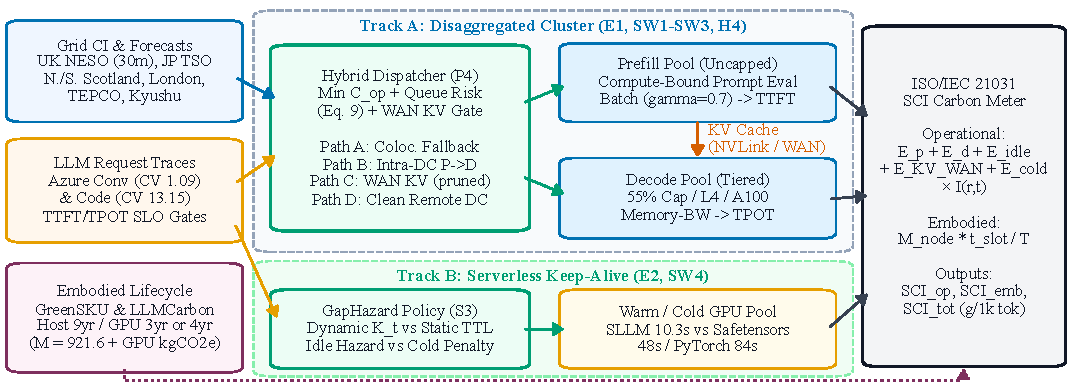
\includegraphics[width=\textwidth]{figures/fig1_architecture.pdf}
    \caption{Dual-track carbon-aware phase-disaggregated LLM cluster (Track A: Paths A--D via Eq.~\eqref{eq:dispatch}) and serverless GPU keep-alive (Track B: GapHazard policy \texttt{S3}) feeding the unified ISO/IEC 21031:2024 SCI telemetry meter.}
    \label{fig:architecture}
\end{figure*}

\subsection{Autoregressive LLM Phases and Disaggregation}\label{subsec:bg_phases}
Within multi-tenant cloud platforms~\cite{mell2011nist}, autoregressive LLM serving proceeds in two stages for each request with prompt length $L_{\text{in}}$ and generation length $L_{\text{out}}$. During \emph{prefill}, the model processes all $L_{\text{in}}$ prompt tokens concurrently through matrix multiplications to produce the first token and populate the KV cache, which determines time-to-first-token (TTFT). During \emph{decode}, the engine iterates token by token over $L_{\text{out}}$ steps, reloading model weights and the growing KV cache from high-bandwidth memory (HBM) on each step; this saturates memory bandwidth before arithmetic units and governs time-per-output-token (TPOT).

Production traces show strong workload skew across domains: Azure LLM logs report conversational prompts averaging $1{,}154.7$ input and $211.1$ output tokens with steady arrivals (coefficient of variation $\text{CV}=1.094$), whereas coding completions average $2{,}047.8$ input and $27.9$ output tokens under extreme burstiness ($\text{CV}=13.152$)~\cite{azure2024trace}. Mooncake traces exhibit even heavier prompt skew, averaging $8{,}590$ input versus $182$ output tokens~\cite{qin2025mooncake}.

Local memory and batching schedulers address single-cluster bottlenecks first. PagedAttention in vLLM cuts KV waste from 61.8\%--79.6\% down to 3.7\% and saves up to 55.2\% KV memory via copy-on-write~\cite{kwon2023vllm}, while Sarathi-Serve uses chunked prefill and stall-free batching to eliminate 28.3$\times$ generation stalls~\cite{agrawal2024sarathi}. Even with chunked batching, colocated requests couple prefill latency spikes with decode tail violations and restrict hardware specialization.

Phase-disaggregated architectures (Splitwise~\cite{patel2024splitwise}, DistServe~\cite{zhong2024distserve}, Mooncake~\cite{qin2025mooncake}, and DualScale~\cite{basit2026dualscale}) separate prefill and decode onto distinct GPU pools connected via NVLink or RDMA fabrics. Splitwise shows that decode GPUs tolerate a 50\% power-cap drop (700~W down to 350~W on H100) with minimal TPOT impact while achieving 2.35$\times$ iso-power-cost throughput~\cite{patel2024splitwise}; DualScale cuts prefill energy by 39\% and decode energy by 48\% at P99 latency parity~\cite{basit2026dualscale}. Empirical measurements confirm that decode still dominates cumulative energy across token ratios~\cite{fernandez2025acl}, and bilinear $(L_{\text{in}}, L_{\text{out}}, L_{\text{in}}L_{\text{out}})$ energy regression achieves $R^2 \ge 0.964$~\cite{wilkins2024offline}. However, recent dual-GPU experiments by Li et al.~\cite{li2026revisiting} caution that disaggregation can underperform colocated inference at small batch sizes over constrained interconnects until batch-32 KV eviction pressure triggers colocation collapse.

\subsection{Wide-Area Carbon Routing and KV Transfer Economics}\label{subsec:bg_wan}
Regional electricity grids vary widely in hourly operational carbon intensity $I(r,t)$ ($\text{gCO}_2\text{eq/kWh}$). Across 123 Electricity Maps grids, Sukprasert et al.~\cite{sukprasert2024limitations} report a 40$\times$ spread (mean $368.39\text{ gCO}_2\text{eq/kWh}$) and note that 87\% of 40 sampled datacenter grids exhibit 24-hour periodicity. Yet latency and capacity constraints sharply curtail pure carbon-chasing: unconstrained 96\% spatial reductions shrink to 51.5\% under 50\% regional spare capacity and 31\% under a \SI{50}{\milli\second} WAN round-trip time (RTT) ceiling, while 50\% grid-forecast error introduces 10\%--12\% overhead~\cite{sukprasert2024limitations}.

Live multi-region Kubernetes scheduling in GreenCourier cuts carbon by 8.7\%--17.8\% across four European zones at a 10.3\%--16.2\% latency penalty~\cite{chadha2023greencourier}, whereas single-cluster temporal deferrals~\cite{wiesner2021letswait}, elastic scaling~\cite{hanafy2023carbonscaler}, battery orchestration~\cite{souza2023ecovisor}, and microservice DAG routing~\cite{gsteiger2024caribou} rely on delay tolerance or small HTTP payloads. In cloud-to-edge continuums, linear-programmed function variant selection lets 30\% more requests satisfy QoS targets and cuts execution carbon by 20\% under equal budgets~\cite{calavaro2026offloading}.

For LLM serving, splitting prefill and decode across WAN regions adds serial KV-cache transmission: a 70B-class FP16 GQA KV state at long context spans hundreds of megabytes per request, adding both WAN transmission latency ($L_{\text{kv}}/B_{\text{wan}}$) and network transfer energy (0.001--0.005~kWh/GB~\cite{gsteiger2024caribou}). Cross-region disaggregation is therefore beneficial only when the carbon savings between regions exceed network transfer emissions without breaching TTFT SLOs.

\subsection{Serverless GPU Keep-Alive and Checkpoint Loading}\label{subsec:bg_serverless}
Under bursty traffic, such as Azure Functions where 81\% of apps see $\le 1\text{ req/min}$~\cite{shahrad2020serverless}, idle servers draw static power while eviction incurs cold-start energy. In Kepler benchmarks, idle CPU draw reaches 21\%--83\% of peak power~\cite{sun2026lacere}, and an idle GPU draws 60--100~W. For 70B-class LLMs (about 130~GB weights), checkpoint cold-start duration spans 84.0~s under standard PyTorch loading, 48.0~s under Safetensors, and 10.3~s even with ServerlessLLM NVMe RAID-0 Direct I/O~\cite{fu2024serverlessllm}.

Recent dynamic keep-alive controllers (EcoLife~\cite{jiang2024ecolife}, CASA~\cite{qi2024casa}, LowCarb~\cite{roy2026lowcarb}, LACE-RL at -77.08\% idle carbon~\cite{sun2026lacere}, and Festina at -56\% energy and -85\% cold starts~\cite{wang2026festina}) show that adaptive idle timeouts outperform fixed windows, yet systematic comparison across multi-gigabyte loader tiers and clean versus coal-heavy grids remains open.

\subsection{ISO/IEC 21031:2024 SCI and Embodied Carbon}\label{subsec:bg_sci}
To prevent shifting emissions between operational and hardware budgets, the Green Software Foundation Software Carbon Intensity (SCI) specification, standardized as ISO/IEC 21031:2024~\cite{iso2024sci}, mandates an additive lifecycle intensity per functional unit $R$ (here, 1,000 processed tokens) while explicitly excluding offset purchases:
\begin{equation}\label{eq:sci}
\text{SCI} = \frac{(E \cdot I) + M}{R},
\end{equation}
where $E$ is total consumed electricity ($\text{kWh}$, inclusive of datacenter PUE), $I$ is regional grid carbon intensity ($\text{gCO}_2\text{eq/kWh}$), and $M = M_{\text{server}} \cdot (t_{\text{slot}}/T_{\text{life}})$ is amortized manufacturing carbon.

Industry GHG audits~\cite{gupta2021chasing}, architectural models~\cite{gupta2022act,acun2023carbonexplorer}, and LLM carbon tools~\cite{faiz2024llmcarbon,li2025ecoserve} show that embodied emissions (800~kgCO$_2$eq host baseline~\cite{li2025ecoserve}; 921.6~kgCO$_2$eq in the GreenSKU Genoa assembly, plus die/HBM~\cite{faiz2024llmcarbon}) represent 24\%--35\% of LLM totals on average grids and surpass 80\% as grids decarbonize. Consequently, metrics using raw GPU utilization~\cite{sinha2025utilization} or ignoring power capping~\cite{kakolyris2025throttllem,stojkovic2025dynamollm,stojkovic2025tapas} and aging amortization~\cite{hewage2025aging,li2023clover} risk optimizing local Watts while raising system-wide lifecycle carbon. These tradeoffs motivate unified simulation testbeds in the tradition of CloudSim~\cite{calheiros2011cloudsim}.

\section{PRISMA-2020-Guided Review Methodology}\label{sec:methodology}

To ground \texttt{RQ1} and parameterize the simulator from primary artifacts, I conducted a PRISMA-2020-guided literature review across Crossref, Semantic Scholar, OpenAlex, arXiv, ACM Digital Library, IEEE Xplore, USENIX, and official standards indices.

\subsection{Search Queries, Inclusion Criteria, and Screening}\label{subsec:prisma_search}
Candidate studies published between 2011 and November 2026 were retrieved across three channels, expanded in revision~v2 with targeted searches over 2024--November 2026 preprints and proceedings:
\begin{itemize}
    \item \textbf{Channel 1 (Carbon-Aware Cloud \& Serverless Scheduling, 16 records):} Paired carbon-intensity, grid emissions, SCI, and embodied terms with spatial/temporal shifting, serverless keep-alive, and cold-start mitigation (\texttt{Query A}).
    \item \textbf{Channel 2 (Phase-Disaggregated LLM Serving \& v2 Update, 44 records):} Combined LLM inference, KV caching, prefill/decode disaggregation, and GPU serving with energy, DVFS, power capping, and embodied/SCI queries (\texttt{Query B}, plus 2024--2026 arXiv/Crossref follow-ups on \texttt{"embodied carbon" AND "LLM" AND "inference"}, \texttt{"serverless" AND "keep-alive" AND "LLM" AND "carbon"}, \texttt{"Software Carbon Intensity" AND "LLM"}, and \texttt{"carbon-aware" + "prefill decode disaggregation"}). Exact boolean search strings and log dates appear in the online supplement.
    \item \textbf{Channel 3 (Surveys, Traces, Lifecycle Models \& Snowballing, 38 records):} Aggregated recent surveys, standards, hardware embodied datasets, citation chasing, and 9 systems verified during revision~v2~\cite{shi2024greenllm,topcu2026tension,sisodia2026sicp,zhang2026context,bernhard2026cleanest,tian2026greencache,moore2025slit,ozcan2025vidurvessim,nguyen2025sustainable}.
\end{itemize}

\textbf{Single-Author and AI-Assisted Screening Protocol:} All candidate retrieval, deduplication, and full-text eligibility checks were performed by a single human author assisted by generative AI search and extraction tooling; every included entry's bibliographic metadata, DOI/arXiv identifier, and quantitative metrics were verified directly against primary PDFs, HTML preprints, or Crossref records. As shown in Fig.~\ref{fig:prisma}, removing 3 duplicates from 98 identified records left 95 unique records for title/abstract screening. Excluding 14 out-of-scope records (lacking cloud serving, datacenter energy, or carbon context, including 3 edge/mobile/satellite works) yielded 81 candidates for eligibility assessment, where 20 more were excluded (offline training only, latency-only disaggregation/pruning, or superseded position notes), leaving 61 included works.

\begin{figure}[t]
    \centering
    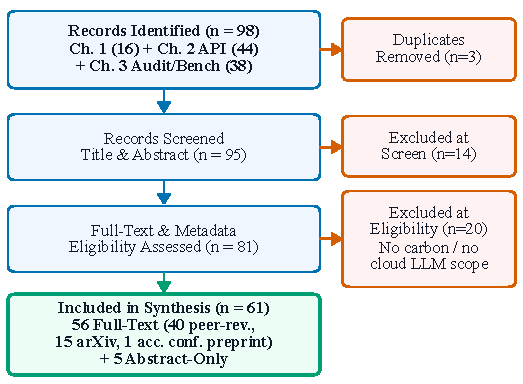
\includegraphics[width=\ifdefined\BUILDELSEVIER 0.85\linewidth\else 0.78\linewidth\fi]{figures/fig2_prisma_flow.pdf}
    \caption{PRISMA-2020-guided search, screening, and eligibility pipeline yielding the 61-work corpus (56 full-text, 5 abstract-only).}
    \label{fig:prisma}
\end{figure}

\subsection{Corpus Provenance and Preprint Disclosure}\label{subsec:corpus_audit}
The 61-work corpus comprises 47 empirical/modeling systems, 11 surveys or research agendas, 2 standards (ISO/IEC 21031:2024~\cite{iso2024sci} and NIST SP 800-145~\cite{mell2011nist}), and 1 trace release~\cite{azure2024trace}. By recency, 56/61 works (91.8\%) appeared in 2022--2026, and 34/61 (55.7\%) appeared in 2025--2026. Retrieval depth breaks down as:
\begin{enumerate}
    \item \textbf{Full-Text Audited (56/61, 91.8\%):} Complete texts underwent equation and table verification, spanning 40 archival publications/standards/traces plus 16 preprints (15 arXiv-only preprints~\cite{hewage2026carbon,yang2025container,pan2025inference,li2025ecoserve,basit2026dualscale,shi2024greenllm,topcu2026tension,sisodia2026sicp,zhang2026context,bernhard2026cleanest,ozcan2025vidurvessim,yan2026pdprov,jegham2025hungryai,zhen2025taming,lu2026etcinfer} and 1 accepted SIGOPS ATC 2026 preprint~\cite{wang2026festina}).
    \item \textbf{Abstract-Only Verified (5/61, 8.2\%):} Five paywalled records relied strictly on verified abstracts~\cite{roy2026lowcarb,calavaro2026offloading,gupta2022act,sinha2025utilization,calheiros2011cloudsim}, with zero constants imported into the simulator.
\end{enumerate}

\section{Taxonomy and Literature Synthesis}\label{sec:taxonomy}

This section answers \texttt{RQ1} by organizing the 47 retained works into six functional classes (\texttt{L1.A--L1.F}) and mapping empirical intersections across phase awareness and carbon/energy signals.

\subsection{Dual-Axis Taxonomy (\texorpdfstring{\texttt{L1.A--L1.F}}{L1.A-L1.F})}\label{subsec:taxonomy_classes}

\subsubsection{L1.A Prior Surveys and Taxonomies (\texorpdfstring{$n=9$}{n=9})}
Recent surveys cover cloud carbon scheduling or LLM efficiency separately without documenting the combined design space (Table~\ref{tab:surveys}). Hewage et al.~\cite{hewage2026carbon} synthesize operational and embodied carbon control for latency-sensitive clouds without mentioning LLMs, prefill/decode, or KV caching. Yang et al.~\cite{yang2025container} review container orchestration across serverless and GPU workloads while omitting disaggregation and embodied carbon. Alam et al.~\cite{alam2026computing} report that 70\% (44/63) of surveyed carbon-aware cloud studies rely solely on simulation and only 6.3\% (4/63) track live grid intensity. Among serverless reviews, Agarwal et al.~\cite{agarwal2026serverless} find sustainability metrics in only 4 of 40 dynamic resource schemes, and Besozzi et al.~\cite{besozzi2025serverless} report 29.5\% GPU support across 122 studies alongside only two carbon mentions.

Conversely, LLM serving surveys by Miao et al.~\cite{miao2025serving}, Jiang et al.~\cite{jiang2026kvcache}, and Pan et al.~\cite{pan2025inference} examine KV transfer and disaggregation without operational or embodied carbon accounting, whereas Bai et al.~\cite{bai2026efficiency} cover operational $\text{PUE}\cdot\text{kWh}\cdot\text{CI}$ metrics without phase disaggregation or embodied manufacturing budgets.

\begin{table*}[t]
\centering
\caption{Audit of Prior Surveys and Taxonomies (\texttt{L1.A}, $n=9$) Across Carbon, Embodied, and LLM Disaggregation Axes}
\label{tab:surveys}
\scriptsize
\setlength{\tabcolsep}{4pt}
\begin{tabular}{@{}llllccccl@{}}
\toprule
\textbf{Work} & \textbf{Year} & \textbf{Venue / Status} & \textbf{Primary Scope} & \textbf{Grid CI} & \textbf{Emb.} & \textbf{LLM} & \textbf{P/D \& KV} & \textbf{Verified Gap Summary} \\
\midrule
Hewage et al.~\cite{hewage2026carbon} & 2026 & arXiv Preprint (28 pp.) & Latency-sensitive cloud & \checkmark & \checkmark & $\times$ & $\times$ & 0 LLM/P/D/KV hits; cites $>60\%$ CO$_2$ cut \\
Yang et al.~\cite{yang2025container} & 2025 & arXiv Preprint (35 pp.) & Container orchestration & \checkmark & $\times$ & Min. & $\times$ & Covers SCI, serverless, GPU; 0 P/D/KV/embodied \\
Alam et al.~\cite{alam2026computing} & 2026 & \textit{Computing} (25 pp.) & Cloud carbon RL/heuristic & 6.3\% & $\times$ & $\times$ & $\times$ & 70\% (44/63) sim-only; 0 GPU/LLM/embodied \\
Agarwal et al.~\cite{agarwal2026serverless} & 2026 & \textit{ACM CSUR} (36 pp.) & Serverless adaptation & 4/40 & $\times$ & Min. & $\times$ & Sustainability secondary; 0 P/D/KV/embodied \\
Besozzi et al.~\cite{besozzi2025serverless} & 2025 & \textit{IEEE Access} (46 pp.) & Serverless architectures & 2 hits & $\times$ & $\times$ & $\times$ & 29.5\% GPU support; 0 LLM/P/D/embodied \\
Miao et al.~\cite{miao2025serving} & 2025 & \textit{ACM CSUR} (35 pp.) & Generative LLM serving & Min. & $\times$ & \checkmark & \checkmark & Covers KV \& disagg; 0 embodied/CI/water \\
Bai et al.~\cite{bai2026efficiency} & 2026 & \textit{ACM CSUR} (70 pp.) & LLM serving efficiency & \checkmark & $\times$ & \checkmark & $\times$ & PUE$\cdot$kWh$\cdot$CI metrics; 0 disagg/cold/embodied \\
Jiang et al.~\cite{jiang2026kvcache} & 2026 & \textit{ACL Findings} (27 pp.) & KV-cache compression & $\times$ & $\times$ & \checkmark & \checkmark & Recommends J/tok; 0 grid CI or embodied \\
Pan et al.~\cite{pan2025inference} & 2025 & arXiv Preprint (25 pp.) & Data-centric LLM systems & $\times$ & $\times$ & \checkmark & \checkmark & 29 prefill, 12 disagg; 0 carbon or energy \\
\bottomrule
\end{tabular}
\end{table*}

\subsubsection{L1.B Spatial and Temporal Cloud Carbon Schedulers (\texorpdfstring{$n=8$}{n=8})}
Temporal delay schedulers such as Wait Awhile (-4.1\% to -11.2\% CO$_2$ within $\pm 8\text{ h}$ windows)~\cite{wiesner2021letswait}, CarbonScaler (-19\% mean AWS savings, -36\% Ontario, -51\% NL)~\cite{hanafy2023carbonscaler}, EcoVisor (-50.05\% BLAST via batteries)~\cite{souza2023ecovisor}, and Clover ($>75\%$ CO$_2$ cut on MIG-partitioned vision/BERT jobs)~\cite{li2023clover} target batch elasticity or multi-second slacks incompatible with interactive token streaming.

Multi-region frameworks including GreenCourier (-8.7\% to -17.8\% carbon at 10.3\%--16.2\% latency increase)~\cite{chadha2023greencourier}, Caribou (-22.9\% to -66.6\% for FaaS DAGs)~\cite{gsteiger2024caribou}, Calavaro et al.~\cite{calavaro2026offloading} (LP edge-cloud offloading yielding +30\% QoS and -20\% carbon under equal budgets, verified from abstract only), and Sukprasert et al.~\cite{sukprasert2024limitations} show regional carbon arbitrage (40x grid spread) alongside RTT and capacity bottlenecks (dropping from a 96\% to a 31\% ceiling under 50~ms WAN RTT). None of the four cross-region schedulers (0/4) models LLM P/D disaggregation or WAN KV serialization.

\subsubsection{L1.C Carbon-Aware Serverless Keep-Alive and Loaders (\texorpdfstring{$n=7$}{n=7})}
Trace characterization on Azure Functions (81\% of apps invoked $\le 1/\text{min}$)~\cite{shahrad2020serverless} motivated dynamic keep-alive controllers. EcoLife cuts idle and operational emissions on multi-generation CPUs within 5.5\% of oracle~\cite{jiang2024ecolife}; CASA jointly balances water and grid CO$_2$ around 15~s Knative cold starts (1.9x--2.8x reduction)~\cite{qi2024casa}; LowCarb applies RL keep-alive control within 15\% of optimal (abstract only)~\cite{roy2026lowcarb}; and LACE-RL uses Kepler idle-power ratios (0.21--0.83) to cut cold starts by 51.7\% and idle carbon by 77.08\%~\cite{sun2026lacere}.

On GPUs, ServerlessLLM shrinks 70B checkpoint loads to 10.3~s via NVMe Direct I/O (48.0~s Safetensors, 84.0~s PyTorch)~\cite{fu2024serverlessllm}, while Festina integrates 3D lookup tables, GPU MPS, DVFS, and early-warning eviction (-56\% energy, -85\% cold starts) alongside a P/D-disaggregated variant (-7\% energy)~\cite{wang2026festina}. Yet neither ServerlessLLM nor Festina evaluates large-checkpoint keep-alive dynamics under grid-intensity extremes.

\subsubsection{L1.D Phase-Disaggregated and Engine-Level LLM Serving (\texorpdfstring{$n=12$}{n=12})}
At the inference engine level, vLLM (cuts KV waste from 61.8\%--79.6\% to 3.7\%)~\cite{kwon2023vllm}, Sarathi-Serve (chunked prefill)~\cite{agrawal2024sarathi}, Wilkins et al.\ (bilinear $(L_{\text{in}}, L_{\text{out}})$ energy modeling, $R^2 \ge 0.964$)~\cite{wilkins2024offline}, and ThrottLL'eM (NVML frequency capping up to -43.8\% energy)~\cite{kakolyris2025throttllem} operate without phase disaggregation. Colocated phase-aware governors (DynamoLLM at -38\% operational carbon~\cite{stojkovic2025dynamollm}, TAPAS at -23\%--24\% row power and +40\% oversubscription~\cite{stojkovic2025tapas}, and Fernandez et al.\ at -37.6\% to -73.0\% energy under vLLM and +55.23\% penalty at TP4~\cite{fernandez2025acl}) tune local frequencies or cluster capacity on a single grid.

Fully disaggregated systems (Splitwise~\cite{patel2024splitwise}, DistServe~\cite{zhong2024distserve}, Mooncake~\cite{qin2025mooncake}, DualScale at -39\% prefill and -48\% decode energy~\cite{basit2026dualscale}, and Li et al.~\cite{li2026revisiting} on small-batch overhead) optimize intra-datacenter throughput or local Watts/Joules (W/J) while omitting grid CI and embodied emissions (0/6 when counting Festina's P/D variant).

\subsubsection{L1.E Embodied Hardware and Lifecycle Models (\texorpdfstring{$n=8$}{n=8})}
Lifecycle studies anchor Scope 3 amortization. Gupta et al.~\cite{gupta2021chasing,gupta2022act} show manufacturing dominates once clean grids exceed 80\% renewables and formalize Reduce/Reuse/Recycle modeling (ACT verified abstract only). CarbonExplorer shows that 100\% annual RECs deliver only 46\%--51\% hourly carbon-free energy~\cite{acun2023carbonexplorer}, while ISO/IEC 21031:2024~\cite{iso2024sci} prohibits offset netting in SCI.

For AI accelerators, LLMCarbon models H100 die and DRAM/SSD embodied emissions (24\%--35\% of serving total)~\cite{faiz2024llmcarbon}, Sinha et al.\ challenge linear utilization-carbon assumptions across co-located workloads and token ratios (abstract only)~\cite{sinha2025utilization}, Hewage et al.\ apply NBTI aging awareness (-37.67\% P99 annualized CPU embodied carbon)~\cite{hewage2025aging}, and EcoServe combines 4R principles (9~yr host / 3~yr GPU lifetimes) for up to 47\% total carbon savings without phase disaggregation or cross-region routing~\cite{li2025ecoserve}.

\subsubsection{L1.F Cloud Standards, Simulation Foundations, and Traces (\texorpdfstring{$n=3$}{n=3})}
NIST SP 800-145 defines multi-tenant resource pooling~\cite{mell2011nist}, CloudSim establishes extensible federated cloud simulation~\cite{calheiros2011cloudsim} (abstract only), and the Azure LLM Inference Trace 2024 supplies \texttt{conv} and \texttt{code} arrival/token distributions~\cite{azure2024trace}.

\subsection{Gap Quantification and Synthesis Matrix}\label{subsec:gap_matrix}
Cross-tabulating the 38 non-survey works in Fig.~\ref{fig:heatmap} identifies exact zero-coverage intersections. All five pure disaggregated systems~\cite{patel2024splitwise,zhong2024distserve,qin2025mooncake,basit2026dualscale,li2026revisiting} plus Festina's P/D variant~\cite{wang2026festina} lie strictly in the Perf/Telem. (2) and Local W/J (4) columns, so 0 works intersect phase disaggregation with either Grid Op. CI or Op. + Embodied. Similarly, only one colocated phase-aware system (DynamoLLM~\cite{stojkovic2025dynamollm}) responds to grid CI, and none (0/4) includes embodied hardware carbon.

Across the complete 47-work corpus (Fig.~\ref{fig:trends}), 37/47 (78.7\%) omit embodied accounting, while empirical evaluations split across physical clusters (14/35, 40.0\%), hybrid testbed-plus-simulators (10/35, 28.6\%), trace simulators/models (9/35, 25.7\%), and abstract-only records (2/35, 5.7\%). Table~\ref{tab:matrix} summarizes how the proposed design integrates these previously disconnected mechanisms.

\begin{figure}[t]
    \centering
    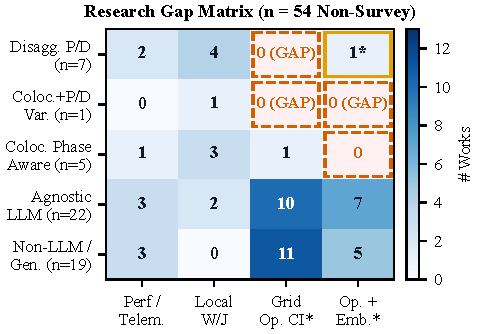
\includegraphics[width=\columnwidth]{figures/fig3_taxonomy_heatmap.pdf}
    \caption{Intersection of phase awareness and carbon/energy signal across $n=38$ non-survey works. *Grid Op. CI includes 10 grid-CI systems plus 2 with battery/water co-signals~\cite{souza2023ecovisor,qi2024casa}; *Op. + Embodied includes 8 operational+embodied works plus CPU aging~\cite{hewage2025aging}.}
    \label{fig:heatmap}
\end{figure}

\begin{figure}[t]
    \centering
    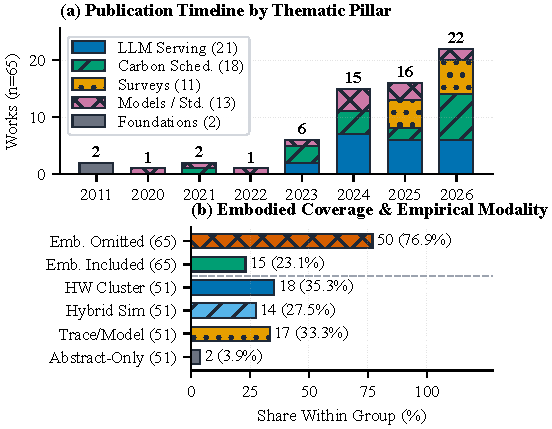
\includegraphics[width=\columnwidth]{figures/fig4_publication_trends.pdf}
    \caption{Corpus bibliometrics from 2011 to 2026 ($n=47$): (a) surge in 2024--2026 output (48.9\% in 2025--2026); (b) 78.7\% embodied omission and empirical evaluation split ($n=35$).}
    \label{fig:trends}
\end{figure}

\begin{table*}[t]
\centering
\caption{Synthesis Comparison Across Empirical Scheduling, LLM Serving, and Lifecycle Carbon Categories (\texttt{L1.B--L1.F})}
\label{tab:matrix}
\scriptsize
\setlength{\tabcolsep}{2.5pt}
\begin{tabular}{@{}p{4.6cm}lllccccp{3.6cm}@{}}
\toprule
\textbf{Category / Representative Works} & \textbf{Class} & \textbf{Scope} & \textbf{Phase} & \textbf{Grid CI} & \textbf{Emb.} & \textbf{KV WAN} & \textbf{Keep-Alive} & \textbf{Primary Knobs / Metrics} \\
\midrule
Wait Awhile~\cite{wiesner2021letswait}, CarbonScaler~\cite{hanafy2023carbonscaler}, EcoVisor~\cite{souza2023ecovisor}, Clover~\cite{li2023clover} & L1.B & Single DC & Non-LLM & \checkmark & $\times$ & $\times$ & $\times$ & Temporal shift, MIG, batteries \\
GreenCourier~\cite{chadha2023greencourier}, Sukprasert~\cite{sukprasert2024limitations}, Caribou~\cite{gsteiger2024caribou}, Calavaro~\cite{calavaro2026offloading}$^\dagger$ & L1.B & Multi-DC & Non-LLM & \checkmark & $\times$ & $\times$ & $\times$ & Geo-routing, HTTP/DAG hops, LP \\
Shahrad~\cite{shahrad2020serverless}, CASA~\cite{qi2024casa}, EcoLife~\cite{jiang2024ecolife}, LowCarb~\cite{roy2026lowcarb}$^\dagger$, LACE-RL~\cite{sun2026lacere}$^\ddagger$ & L1.C & Serverl. & Non-LLM & \checkmark & EcoLife & $\times$ & \checkmark & Dynamic TTL, water+CI, DQN \\
ServerlessLLM~\cite{fu2024serverlessllm}, Festina~\cite{wang2026festina}$^\ddagger$ & L1.C & Serverl. & Agnostic/P/D & $\times$ & $\times$ & $\times$ & \checkmark & NVMe Direct I/O, MPS, DVFS \\
vLLM~\cite{kwon2023vllm}, Sarathi~\cite{agrawal2024sarathi}, Wilkins~\cite{wilkins2024offline}, ThrottLL'eM~\cite{kakolyris2025throttllem} & L1.D & Engine & Agnostic/Col. & $\times$ & $\times$ & $\times$ & $\times$ & PagedAttn, chunking, NVML cap \\
DynamoLLM~\cite{stojkovic2025dynamollm}, TAPAS~\cite{stojkovic2025tapas}, Fernandez et al.~\cite{fernandez2025acl} & L1.D & Cluster & Coloc.\ Phase & Dynamo & $\times$ & $\times$ & $\times$ & Multi-loop DVFS, TP, power cap \\
Splitwise~\cite{patel2024splitwise}, DistServe~\cite{zhong2024distserve}, Mooncake~\cite{qin2025mooncake}, DualScale~\cite{basit2026dualscale}$^\ddagger$, Li~\cite{li2026revisiting}$^\ddagger$ & L1.D & Intra-DC & Disagg.\ P/D & $\times$ & $\times$ & Intra-DC & $\times$ & P/D pools, 50\% cap, MPC, RDMA \\
Gupta~\cite{gupta2021chasing,gupta2022act}$^\dagger$, CarbonExplorer~\cite{acun2023carbonexplorer}, LLMCarbon~\cite{faiz2024llmcarbon}, ISO~\cite{iso2024sci}, Sinha~\cite{sinha2025utilization}$^\dagger$ & L1.E & Lifecycle & Agnostic/Gen. & \checkmark & \checkmark & $\times$ & $\times$ & SCI Eq.~\eqref{eq:sci}, die/HBM capex \\
EcoServe~\cite{li2025ecoserve}$^\ddagger$, Hewage et al.~\cite{hewage2025aging} & L1.E & Cluster & Agnostic & \checkmark & \checkmark & $\times$ & $\times$ & 4R lifetimes (9/3~yr), NBTI aging \\
NIST~\cite{mell2011nist}, CloudSim~\cite{calheiros2011cloudsim}$^\dagger$, Azure Trace~\cite{azure2024trace} & L1.F & Found. & Spec./Trace & $\times$ & $\times$ & $\times$ & $\times$ & Taxonomy, Cloud sim, conv/code logs \\
\midrule
\textbf{This Work (\texttt{P4} Cluster + \texttt{S3} Serverless)} & \text{--} & \textbf{Multi-DC} & \textbf{Disagg.\ P/D} & \checkmark & \checkmark & \checkmark & \checkmark & \textbf{Hybrid A--D, SCI, GapHazard} \\
\bottomrule
\multicolumn{9}{@{}l@{}}{\scriptsize $^\dagger$Abstract-only verified (5 works in corpus). $^\ddagger$Preprint / accepted conference preprint (EcoServe, DualScale, Li et al., LACE-RL, Festina).}
\end{tabular}
\end{table*}

\section{Simulation Architecture and Experimental Design}\label{sec:sim_design}

\subsection{Parameterized Simulation Scope Statement}\label{subsec:scope_statement}
All empirical results derive from a parameterized SimPy 4.1.2 discrete-event simulator without physical multi-continent GPU cluster telemetry; consistent with Alam et al.~\cite{alam2026computing} (70\% simulation-based cloud carbon studies), this enables controlled multi-seed ablations across heterogeneous grids. Constants split into published baselines (Table~\ref{tab:params}) and explicit calibration assumptions (Supplement Table~S6), driven by CC-BY-4.0 traces.

\subsection{Phase Execution, Power, and Dispatch Formulation}\label{subsec:sim_equations}

For request $i$ arriving at time $t_i$ with prompt length $L_{\text{in}}(i)$ and output length $L_{\text{out}}(i)$, prefill duration on GPU tier $g$ scales linearly above base kernel overhead $\tau_{P,0}(g)$:
\begin{equation}\label{eq:prefill_lat}
T_{\text{exec},P}(i,g) = \tau_{P,0}(g) + \tau_{P,\text{tok}}(g)\cdot L_{\text{in}}(i),
\end{equation}
calibrated to Splitwise Table IV uncontended Llama-70B anchors (\SI{84}{\milli\second} conv and \SI{95}{\milli\second} code on H100; \SI{155}{\milli\second} and \SI{185}{\milli\second} on A100)~\cite{patel2024splitwise}. During continuous-batching decode over active resident KV size $K_{\text{res}}$ (GB) on $G_r$ tensor-parallel GPUs, step time increases with HBM bandwidth contention:
\begin{equation}\label{eq:decode_step}
t_{\text{step}}(g, K_{\text{res}}) = \tau_{D,0}(g) \left(1 + \alpha_{\text{mem}}(g)\frac{K_{\text{res}}}{G_r\,\text{BW}_{\text{HBM}}(g)}\right),
\end{equation}
anchored to \SI{28}{\milli\second} on H100 and \SI{42}{\milli\second} on A100~\cite{patel2024splitwise,stojkovic2025dynamollm}, with mild step inflation only if decode TDP cap $c_{\text{cap}} < 0.50$. Under colocation (\texttt{B1}), concurrent prefill slows active decode progress to factor $r_{\text{coloc}}=0.20$~\cite{agrawal2024sarathi,patel2024splitwise}, whereas disaggregation isolates decode iterations. End-to-end metrics aggregate cold-start delay, queueing, execution, KV transfer, and RTT:
\begin{equation}\label{eq:slo_metrics}
\begin{aligned}
\text{TTFT}_i &= T_{\text{cold},i} + T_{\text{q},P,i} + T_{\text{exec},P,i} + T_{\text{kv},i} + \text{RTT}_i, \\
\text{TPOT}_i &= \frac{T_{D,\text{exit},i} - T_{D,\text{enter},i}}{L_{\text{out}}(i)}.
\end{aligned}
\end{equation}

Instantaneous per-GPU power scales sublinearly with Model FLOPs Utilization ($\text{mfu}$) and active power cap ratio $c_{\text{cap}} \in (0, 1]$ ($c_{\text{cap}}=1.0$ on prefill; $c_{\text{cap}}=0.55$ on decode~\cite{patel2024splitwise}), plus GreenSKU Genoa host ancillary draw $P_{\text{host}}(\text{mfu})$:
\begin{equation}\label{eq:power}
\begin{aligned}
P_{\text{gpu}}(\text{mfu}, c_{\text{cap}}) ={}& P_{\text{idle}} + \left(c_{\text{cap}} P_{\text{TDP}} - P_{\text{idle}}\right) \\
&\times \left(\min\!\left(1.0, \frac{\text{mfu}}{\text{mfu}_{\text{sat}}}\right)\right)^{\gamma},
\end{aligned}
\end{equation}
using saturation threshold $\text{mfu}_{\text{sat}}=0.45$ and calibrated sublinear exponent $\gamma=0.70$.

For Llama-2-70B FP16 GQA-8 ($s_{\text{kv}}=0.3125$~MB/tok), total KV payload $S_{\text{kv}}(i) = s_{\text{kv}} L_{\text{in}}(i)$ transfers over intra-DC NVLink/IB ($\delta_{\text{layer}} \in \{5,8\}\text{ ms}$~\cite{patel2024splitwise}, $\text{BW}_{\text{local}}=400$~Gbps) or cross-region WAN:
\begin{equation}\label{eq:kv_tx}
\begin{aligned}
T_{\text{kv}}(r_P, r_D) &= \text{RTT}(r_P, r_D) + \frac{8 S_{\text{kv}}}{B_{\text{wan}}}, \\
E_{\text{kv}} &= P_{\text{net}}\frac{8 S_{\text{kv}}}{3.6\times 10^6 B_{\text{wan}}}\,\text{PUE}.
\end{aligned}
\end{equation}
Cross-region pipelined disaggregation (Path C from $r_P$ to $r_D \neq r_P$) is admissible only if both a latency recomputation crossover condition and an operational carbon crossover condition hold:
\begin{align}
T_{\text{kv}}(r_P, r_D) + T_{\text{q},D}(r_D) &< \min\!\big(T_{\text{q},D}(r_P),\nonumber\\
&\qquad T_{\text{recomp}}(L_{\text{in}}, r_D)\big), \label{eq:cross_lat}\\
E_P I_{r_P}(t) + E_{\text{kv}}\frac{I_{r_P}(t)+I_{r_D}(t)}{2} &\nonumber\\
+\, E_D I_{r_D}(t) &< \hat{C}_{\text{local}}(i). \label{eq:cross_carb}
\end{align}
Across all feasible paths $p \in \{\text{A: Coloc.},\allowbreak\ \text{B: Intra P/D},\allowbreak\ \text{C: Cross P/D},\allowbreak\ \text{D: Remote Clean DC}\}$ meeting TTFT slack ($0.85\cdot\text{TTFT}_{\text{SLO}}$), hybrid router \texttt{P4} selects:
\begin{equation}\label{eq:dispatch}
\begin{aligned}
p^* = \arg\min_{p \in \mathcal{F}(i,t)} \Big[ &w_c \hat{C}_{\text{op}}(p,t) \\
&+ 40\,w_q \max\!\big(0,\, \text{occ}_D(p) - 0.60\big)^2 \Big],
\end{aligned}
\end{equation}
with $w_c=1.0$, $w_q=0.15$, and decode pool occupancy $\text{occ}_D$; when bursts exceed slack, \texttt{P4} falls back locally to Path A or Path B.

In Track B (serverless GPU serving), an online causal EWMA tracker (\texttt{OnlineGapHazardTracker}, \texttt{S3}) estimates discrete inter-arrival gap probabilities $\mathbf{p}$ across bins $[0\text{--}1, 1\text{--}5, 5\text{--}10, 10\text{--}30, 30\text{--}60, >60]\text{ s}$ and selects dynamic keep-alive timeout $k^* \in \{1, 5, 10, 30, 60\}\text{ s}$~\cite{sun2026lacere} at idle entry:
\begin{equation}\label{eq:gaphazard}
\begin{aligned}
k^*(t) &= \arg\min_{k \in \mathcal{K}} \bigg[ \mathbb{E}[\tau_{\text{idle}}(k)]\, r_{\text{idle}}(t) \\
&\quad + p_{\text{miss}}(k)\!\left(C_{\text{cold}}(t) + \frac{\beta_{\text{SLO}}\,\mathbb{I}_{\text{SLO}}}{\max(\widetilde{I}_r(t), 0.04)}\right) \bigg],
\end{aligned}
\end{equation}
where $r_{\text{idle}}(t)$ is per-second warm-idle carbon rate ($\lambda_{\text{idle}}=0.20$ baseline~\cite{sun2026lacere} or hardware idle ratio), $C_{\text{cold}}(t)$ is reload carbon during $T_{\text{cold}}$, and $\widetilde{I}_r(t)$ is normalized regional intensity.

Finally, operational emissions $C_{\text{op}}$ integrate node and WAN power multiplied by $\text{PUE}=1.12$ and regional grid CI $I_r(t)$, while amortized embodied emissions $C_{\text{emb}}$ sum host and GPU footprints over lifetimes $\text{LT}_{\text{host}}, \text{LT}_{\text{gpu}}$ (4~yr uniform; sensitivity 9~yr host / 3~yr GPU~\cite{li2025ecoserve}):
\begin{equation}\label{eq:emb_sci}
\begin{aligned}
C_{\text{emb}} &= \sum_{m \in \mathcal{N}} \left(\frac{M_{\text{host},m}}{\text{LT}_{\text{host}}} + \frac{G_m M_{\text{gpu},m}}{\text{LT}_{\text{gpu}}}\right) T_{\text{sim}}, \\
\text{SCI}_{\text{tot}} &= \frac{C_{\text{op}} + C_{\text{emb}}}{N_{\text{tok}}/1000}.
\end{aligned}
\end{equation}

\subsection{Verified Baselines, Traces, and Calibrated Assumptions}\label{subsec:traces_params}
Table~\ref{tab:params} lists verified hardware and loader parameters, while non-measured assumptions (RTTs 0.5--200~ms, 10--400~Gbps WAN, $\gamma=0.70$, $f_{\text{cold}}=0.65$, 24h tiling) appear in Supplement Table~S6 and sweeps \texttt{SW1--SW6}. Cluster experiments (\texttt{E1}) span 3 zones (6 nodes, 24 H100s; 2 nodes/region): \texttt{South Scotland} (mean 9.75~gCO$_2$eq/kWh, 0--129), \texttt{London} (163.32, 13--326), and \texttt{TEPCO} (581.64, 302.3--671.5), from Oct.\ 2025 UK NESO ($1{,}344$ 30-min slots) and FY2024 Japan TSO traces ($17{,}520$ slots, scaled $\times 1{,}000$). Azure LLM conversational (\texttt{conv}: $19{,}366$ reqs, 5.53~RPS, $\text{CV}=1.094$, $1{,}154.7$ in / $211.1$ out) and coding (\texttt{code}: $8{,}819$ reqs, 2.57~RPS, $\text{CV}=13.152$, $2{,}047.8$ in / $27.9$ out) traces~\cite{azure2024trace} use DynamoLLM SLOs (250/100, 400/100, 2,000/100~ms TTFT/TPOT)~\cite{stojkovic2025dynamollm}.

Cluster runs compare five routing policies: \texttt{B1} (carbon-agnostic colocated round-robin), \texttt{B2} (intra-region P/D, 55\% decode cap), \texttt{P3} (unconditional cross-region P/D when $\text{RTT} \le \text{TTFT slack}$), \texttt{P4} (hybrid Eqs.~\eqref{eq:cross_lat} through~\eqref{eq:dispatch}), and \texttt{P5} (oracle 30-min grid lookahead).

Serverless runs (\texttt{E2}) compare \texttt{S1} ($0\text{ s}$), \texttt{S2} ($30\text{ s}$), \texttt{S2b} ($60\text{ s}$), and \texttt{S3} (GapHazard Eq.~\eqref{eq:gaphazard}) across \texttt{TEPCO}, \texttt{North Scotland} (mean 35.65~gCO$_2$eq/kWh, std 82.50, 0--355), and \texttt{South Scotland} using ServerlessLLM's \SI{10.3}{\second} 70B loader. Additional robustness sweeps probe Path C activation across $10\text{--}400\text{ Gbps}$ WAN and $5\text{--}200\text{ ms}$ RTT (\texttt{SW5}, 690 runs) and clean scale-out break-even demand from $1.0\times$ to $3.0\times$ RPS (\texttt{SW6}, 560 runs). All suites run across 10 seeds (100--109) and report Student-$t$ 95\% CIs ($t_{0.975,9}=2.262$) and two-sided paired Wilcoxon $p$-values ($\alpha=0.05$, exact floor $p = 2/2^{10} \approx 0.00195$).

\begin{table}[t]
\centering
\caption{Verified Hardware, Embodied, and Loader Parameters}
\label{tab:params}
\scriptsize
\setlength{\tabcolsep}{3pt}
\begin{tabular}{@{}>{\raggedright\arraybackslash}p{2.15cm}>{\raggedright\arraybackslash}p{4.35cm}l@{}}
\toprule
\textbf{Component} & \textbf{Verified Value(s)} & \textbf{Source} \\
\midrule
H100 SXM5 (4/node) & TDP \SI{700}{\watt}, Idle \SI{60}{\watt}, HBM 3352~GB/s, 124.9~kgCO$_2$e & \cite{patel2024splitwise,li2025ecoserve} \\
A100 SXM4 (4/node) & TDP \SI{400}{\watt}, Idle \SI{100}{\watt}, HBM 2039~GB/s, 121.5~kgCO$_2$e & \cite{patel2024splitwise,li2025ecoserve} \\
L4 Decode (8/node) & TDP \SI{72}{\watt}, Idle \SI{14.4}{\watt}, 300~GB/s, 41.2~kgCO$_2$e & \cite{li2025ecoserve} \\
GreenSKU Genoa & Peak \SI{562.4}{\watt}, Idle \SI{164.6}{\watt}, 921.6~kgCO$_2$e & \cite{azure2024trace,li2025ecoserve} \\
Decode Cap \& KV & $c_{\text{cap}}=0.55$; $\delta_{\text{layer}}=5/8\text{ ms}$; PUE $1.12$ & \cite{patel2024splitwise} \\
70B / 13B Loaders & SLLM 10.3 / 2.0~s; Safe 48.0 / 8.2~s; PyT 84.0 / 14.0~s & \cite{fu2024serverlessllm} \\
Amortization Life & Uniform 4~yr; Asymmetric 9~yr host / 3~yr GPU & \cite{li2025ecoserve,gupta2021chasing} \\
\bottomrule
\end{tabular}
\end{table}

\subsection{Simulator Calibration and Held-Out Validation}\label{subsec:validation}
Prior to multi-region sweeps, 24 checks (\texttt{validate\_simulator.py}; Supplement Table~S2) separate 19 \emph{calibration anchors} from 5 \emph{held-out validation checks}. Across the 19 anchors calibrated to Splitwise Table~IV and Figs.~8--9~\cite{patel2024splitwise} plus ServerlessLLM Fig.~6a~\cite{fu2024serverlessllm}, uncontended H100 TPOT (0.00\% \texttt{conv}, -9.68\% \texttt{code}), loader times (0.00\% across 2.0--84.0~s), and 50\%--100\% TDP step stability (4.47\% step delta; +6.0\% below 50\%) match by construction; as an explicit modeling limitation, modeled TTFT deviates by \textbf{13.73\%--14.24\%} on H100 (95.96/108.04 vs.\ 84.0/95.0~ms) and \textbf{8.81\%--9.50\%} on A100 (169.73/201.29 vs.\ 155.0/185.0~ms) due to fixed 5--8~ms transfer stalls. Across the 5 held-out \texttt{conv} checks (0.25x--2.00x RPS), unfitted runs reproduce Li et al.~\cite{li2026revisiting}: \texttt{B2} vs.\ \texttt{B1} energy drops from -20.01\% (0.25x) to -30.40\% (1.50x) as P95 TTFT rises +11.4\% to +44.3\% (2.00x) and P95 TPOT improves -7.8\% to -31.6\%.

\subsection{24-Hour Trace-Tiling Sensitivity Ablation}\label{subsec:tiling_ablation}
Because raw Azure traces span 58.36~min (\texttt{conv}) and 57.27~min (\texttt{code}), I tested 24h block-tiling sensitivity across four modes ($N=10$ \texttt{conv} seeds; \texttt{run\_tiling\_ablation.py}, full 12-row results in Supplement Table~S3). Relative \texttt{P4} $\text{SCI}_{\text{op}}$ savings stay invariant within 0.12~pp (60.70\%--60.82\% vs.\ \texttt{B1}; 44.07\%--44.33\% vs.\ \texttt{B2}), and SLO violations hold within 0.817\%--0.835\% across original 280~s replacement, 280~s no-replacement permutation, fine 90~s, and coarse 900~s regimes.

\section{Simulation Results and Discussion}\label{sec:results}

Unless noted otherwise, all inferential comparisons span $N=10$ paired random seeds ($100\text{--}109$). Because $p = 2/2^{10} \approx 0.002$ ($0.00195$) is the minimum attainable two-sided exact paired Wilcoxon signed-rank $p$-value for $N=10$ whenever all 10 seed pairs agree in sign (rank-biserial correlation $|r_{\text{rb}}| = 1.000$), I report paired mean differences ($\Delta$), Student-$t$ 95\% confidence intervals, rank-biserial $r_{\text{rb}}$, and paired Cohen's $d_z$ alongside exact $p$-values (full paired statistics appear in the online supplement).

\subsection{E1: Multi-Region Cluster Carbon--SLO Frontier}\label{subsec:res_e1}
Table~\ref{tab:e1_results} and Fig.~\ref{fig:e1_pareto} summarize \texttt{E1} across 1h and 24h horizons. On conversational traffic (\texttt{conv}), hybrid routing \texttt{P4} lowers $\text{SCI}_{\text{op}}$ by 60.77\% at 1h ($\Delta = -0.05124$ [-0.05473, -0.04775] g/1k tok, $r_{\text{rb}} = -1.000$, $d_z = -10.50$, $p = 0.002$) and 60.70\% at 24h ($\Delta = -0.04948$ [-0.05220, -0.04676], $d_z = -13.01$, $p = 0.002$) relative to carbon-agnostic colocation \texttt{B1}, and by 43.95\%--44.07\% relative to intra-region phase disaggregation \texttt{B2} ($d_z \in [-19.99, -11.29]$, $p = 0.002$). Because fixed hardware amortization adds $\text{SCI}_{\text{emb}} \approx 0.0090$~gCO$_2$eq/1k tok across equal-capacity clusters, total $\text{SCI}_{\text{tot}}$ drops 54.92\% (1h) and 54.64\% (24h) versus \texttt{B1} at 0.81\%--0.82\% SLO violations (TTFT P95 = 504.5--506.4~ms), well below the 5\% boundary.

By contrast, unconditional spatial disaggregation \texttt{P3} reaches lower $\text{SCI}_{\text{tot}}$ (0.03858 at 24h) at the cost of tail degradation, breaching 5\% at 24h (5.90\% violations, TTFT P95 = 1,190.4~ms). \texttt{P4} cuts \texttt{P3} SLO violations by 83.57\% (1h, $\Delta = -4.12\text{ pp}$ [-5.12, -3.11]) and 86.04\% (24h, $\Delta = -5.08\text{ pp}$ [-6.16, -4.00], $r_{\text{rb}} = -1.000$, $p = 0.002$) for a +6.48\%--6.79\% $\text{SCI}_{\text{tot}}$ trade-off, supporting \textbf{H1} and \textbf{H2}.

\begin{figure*}[t]
    \centering
    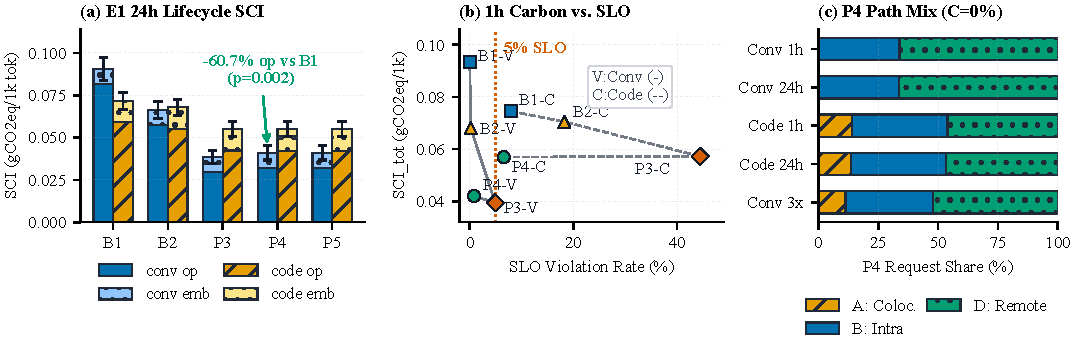
\includegraphics[width=\ifdefined\BUILDELSEVIER 0.94\textwidth\else 0.58\textwidth\fi]{figures/fig5_e1_pareto_paths.pdf}
    \caption{Experiment \texttt{E1} cluster evaluation ($N=10$ seeds, 95\% Student-$t$ CIs): (a) 24h operational plus embodied SCI; (b) 1h carbon--SLO frontier against the 5\% boundary; (c) adaptive \texttt{P4} path mix showing Path C pruned to 0\% at 10~Gbps WAN.}
    \label{fig:e1_pareto}
\end{figure*}

\begin{table*}[t]
\centering
\caption{Experiment \texttt{E1} Multi-Region Cluster Metrics (Mean $\pm$ 95\% CI, $N=10$ Seeds; Paired vs.\ \texttt{P4})}
\label{tab:e1_results}
\scriptsize
\setlength{\tabcolsep}{2.6pt}
\ifdefined\BUILDELSEVIER\resizebox{\textwidth}{!}{\fi
\begin{tabular}{@{}llcccccc@{}}
\toprule
\textbf{Case} & \textbf{Policy} & $\textbf{SCI}_{\text{op}}$ \textbf{(g/1k)} & $\textbf{SCI}_{\text{tot}}$ \textbf{(g/1k)} & \textbf{TTFT P95 (ms)} & \textbf{SLO (\%)} & \textbf{Effect ($r_{\text{rb}}, p$)} & \textbf{Verdict (H1/H2)} \\
\midrule
1h Conv & \texttt{B1} (Coloc.) & $0.08431 \pm 0.00681$ & $0.09329 \pm 0.00681$ & $268.6 \pm 0.0$ & $0.0005 \pm 0.001$ & $-1.00, 0.002$ (op) & Baseline \\
1h Conv & \texttt{B2} (Intra P/D) & $0.05901 \pm 0.00472$ & $0.06799 \pm 0.00472$ & $300.3 \pm 0.2$ & $0.20 \pm 0.04$ & $-1.00, 0.002$ (op) & Baseline \\
1h Conv & \texttt{P3} (Uncond.) & $0.03040 \pm 0.00306$ & $0.03938 \pm 0.00306$ & $1062.3 \pm 136.1$ & $4.93 \pm 1.02$ & $-1.00, 0.002$ (SLO) & Tail Degrad. \\
1h Conv & \texttt{P4} (Hybrid) & $\mathbf{0.03307 \pm 0.00365}$ & $\mathbf{0.04205 \pm 0.00365}$ & $\mathbf{506.4 \pm 2.1}$ & $\mathbf{0.81 \pm 0.06}$ & \text{--} & \textbf{SUPPORTED} \\
\midrule
24h Conv & \texttt{B1} / \texttt{B2} & $0.08150$ / $0.05726$ & $0.09055$ / $0.06631$ & $268.6$ / $300.3$ & $0.00$ / $0.20$ & $-1.00, 0.002$ (op) & Baselines \\
24h Conv & \texttt{P3} (Uncond.) & $0.02953 \pm 0.00369$ & $0.03858 \pm 0.00371$ & $1190.4 \pm 156.0$ & $5.90 \pm 1.10$ & $-1.00, 0.002$ (SLO) & Breaches 5\% \\
24h Conv & \texttt{P4} (Hybrid) & $\mathbf{0.03203 \pm 0.00434}$ & $\mathbf{0.04108 \pm 0.00436}$ & $\mathbf{504.5 \pm 3.7}$ & $\mathbf{0.82 \pm 0.03}$ & \text{--} & \textbf{SUPPORTED} \\
\midrule
1h Code & \texttt{B1} / \texttt{B2} & $0.06182$ / $0.05773$ & $0.07457$ / $0.07048$ & $592.8$ / $3209.1$ & $7.91$ / $18.25$ & $-1.00, 0.002$ (op) & CV 13.15 \\
1h Code & \texttt{P3} (Uncond.) & $0.04441 \pm 0.00385$ & $0.05722 \pm 0.00385$ & $39317.8 \pm 793.9$ & $44.45 \pm 0.28$ & $-1.00, 0.002$ (SLO) & WAN Collapse \\
1h Code & \texttt{P4} (Hybrid) & $\mathbf{0.04419 \pm 0.00388}$ & $\mathbf{0.05694 \pm 0.00388}$ & $\mathbf{1613.8 \pm 4.3}$ & $\mathbf{6.57 \pm 0.25}$ & \text{--} & \textbf{H1 Part./H2 Sup.} \\
\midrule
24h Code & \texttt{B1}/\texttt{B2}/\texttt{P3} & $0.05911$/$0.05525$/$0.04235$ & $0.07171$/$0.06784$/$0.05495$ & $612.5$/$3380$/$30725$ & $8.46$/$19.47$/$44.57$ & $\le -0.82, \le 0.020$ & Baselines \\
24h Code & \texttt{P4} / \texttt{P5} & $\mathbf{0.04226}$ / $0.04226$ & $\mathbf{0.05485}$ / $0.05485$ & $\mathbf{1598.9}$ / $1599.0$ & $\mathbf{6.24}$ / $6.23$ & $|r_{\text{rb}}| \le 0.20, \ge 0.652$ & \textbf{H1 Part./H2 Sup.} \\
\bottomrule
\end{tabular}%
\ifdefined\BUILDELSEVIER}\fi
\end{table*}

Under bursty coding completions (\texttt{code}, $\text{CV}=13.152$, mean $2{,}047.8$-token prompts; Fig.~\ref{fig:e1_pareto}b), \texttt{P4} cuts $\text{SCI}_{\text{op}}$ by 28.51\% versus \texttt{B1} ($\Delta = -0.01763$ [1h], $-0.01685$ [24h], $d_z \in [-13.14, -9.73]$, $p = 0.002$) and 23.45\%--23.51\% versus \texttt{B2} ($p = 0.002$). Unconditional \texttt{P3} saturates the WAN with 192.5--193.1~GB/1k-req KV transfers, driving SLO violations to 44.45\%--44.57\% (TTFT P95 = 30.7--39.3~s). To trace where spatial gains originate, \texttt{P4}'s gates prune cross-region Path C cleanly to \textbf{0.00\%} at 10--25~Gbps (Section~\ref{subsec:res_sweeps}). Consequently, \texttt{P4}'s operational carbon reductions come primarily from \textbf{Path D} (whole-request remote clean-grid execution: 66.13\%--66.27\% on \texttt{conv}, 46.08\%--46.74\% on \texttt{code}) paired with local intra-DC fallbacks onto Path B (33.54\%--39.81\%) and Path A (0.20\%--14.11\%), cutting \texttt{P3}'s \texttt{code} SLO violations by 85.22\% (1h, $\Delta = -37.88\text{ pp}$ [-38.21, -37.55], $d_z = -82.83$, $p = 0.002$) and 86.01\% (24h, $\Delta = -38.34\text{ pp}$ [-38.57, -38.10], $d_z = -118.80$). Oracle 30-min grid lookahead \texttt{P5} matches \texttt{P4} within 0.02\% on carbon and 0.25\% on SLOs ($p \ge 0.160$).

\subsection{\texorpdfstring{E2 \& SW4}{E2 and SW4}: Serverless Keep-Alive and Loader Sensitivity}\label{subsec:res_e2}
Table~\ref{tab:e2_results} and Fig.~\ref{fig:e2_serverless} reveal an inverse regional trade-off for dynamic keep-alive (\texttt{S3}). On carbon-intensive \texttt{TEPCO} (581.6~gCO$_2$eq/kWh), 24h GapHazard \texttt{S3} achieves the lowest operational intensity ($\text{SCI}_{\text{op}}=0.10825$), trimming operational carbon by 8.05\% below scale-to-zero \texttt{S1} ($\Delta=-0.00948$ [-0.01058, -0.00838], $r_{\text{rb}}=-1.000$), 7.03\% below 30~s static \texttt{S2} ($\Delta=-0.00819$ [-0.00873, -0.00764]), and 11.02\% below 60~s \texttt{S2b} ($\Delta=-0.01340$, all $p=0.002$). However, aggressive dirty-slot eviction leaves 28.60\% SLO violations (4,529 cold starts) versus 19.45\% (\texttt{S2}) and 13.03\% (\texttt{S2b}), though well below \texttt{S1} (40.25\%), partially supporting \textbf{H3}.

\begin{figure*}[t]
    \centering
    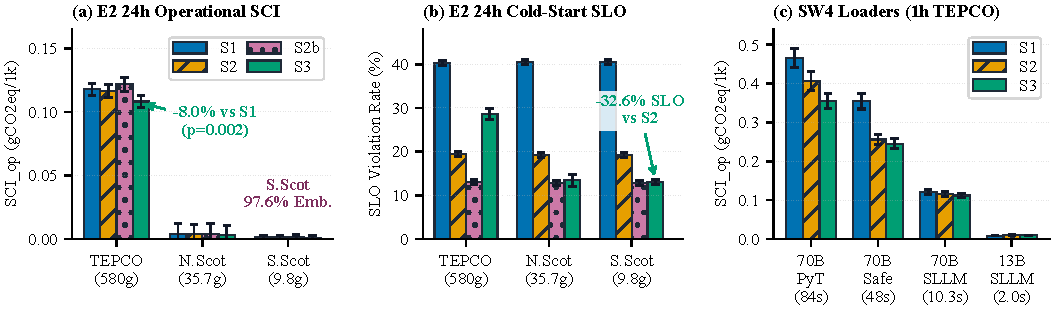
\includegraphics[width=\ifdefined\BUILDELSEVIER 0.94\textwidth\else 0.58\textwidth\fi]{figures/fig6_e2_serverless.pdf}
    \caption{Experiment \texttt{E2} and \texttt{SW4} serverless evaluation ($N=10$ seeds, 95\% CIs): (a) 24h operational SCI; (b) 24h cold-start SLO violations across grid intensities; (c) \texttt{SW4} loader sensitivity (84~s PyTorch down to 10.3~s ServerlessLLM and 2.0~s 13B).}
    \label{fig:e2_serverless}
\end{figure*}

\begin{table}[t]
\centering
\caption{Experiment \texttt{E2} 24h Serverless Keep-Alive Metrics ($N=10$ Seeds)}
\label{tab:e2_results}
\scriptsize
\setlength{\tabcolsep}{2.4pt}
\begin{tabular}{@{}llcccc@{}}
\toprule
\textbf{Region} & \textbf{Pol.} & $\textbf{SCI}_{\text{op}}$ & \textbf{Emb.\ (\%)} & \textbf{SLO (\%)} & \textbf{Cold Starts} \\
\midrule
\texttt{TEPCO} & \texttt{S1} ($0\text{ s}$) & $0.11773$ & $22.2$ & $40.25$ & $6{,}271.6$ \\
\texttt{TEPCO} & \texttt{S2} ($30\text{ s}$) & $0.11644$ & $22.4$ & $19.45$ & $3{,}054.7$ \\
\texttt{TEPCO} & \texttt{S2b} ($60\text{ s}$) & $0.12166$ & $21.6$ & $\mathbf{13.03}$ & $2{,}081.0$ \\
\texttt{TEPCO} & \texttt{S3} (GapHaz.) & $\mathbf{0.10825}$ & $23.7$ & $28.60$ & $4{,}529.0$ \\
\midrule
\texttt{N.\ Scot.} & \texttt{S1} ($0\text{ s}$) & $0.00373$ & $94.6$ & $40.48$ & $6{,}373.4$ \\
\texttt{N.\ Scot.} & \texttt{S2} ($30\text{ s}$) & $0.00362$ & $94.7$ & $19.29$ & $3{,}069.1$ \\
\texttt{N.\ Scot.} & \texttt{S2b} ($60\text{ s}$) & $0.00378$ & $94.6$ & $\mathbf{12.84}$ & $2{,}073.4$ \\
\texttt{N.\ Scot.} & \texttt{S3} (GapHaz.) & $\mathbf{0.00323}$ & $\mathbf{95.0}$ & $13.40$ & $2{,}164.8$ \\
\midrule
\texttt{S.\ Scot.} & \texttt{S1} ($0\text{ s}$) & $0.00106$ & $97.4$ & $40.48$ & $6{,}373.4$ \\
\texttt{S.\ Scot.} & \texttt{S2} ($30\text{ s}$) & $0.00103$ & $97.4$ & $19.29$ & $3{,}069.1$ \\
\texttt{S.\ Scot.} & \texttt{S2b} ($60\text{ s}$) & $0.00108$ & $97.4$ & $\mathbf{12.84}$ & $2{,}073.4$ \\
\texttt{S.\ Scot.} & \texttt{S3} (GapHaz.) & $\mathbf{0.00094}$ & $\mathbf{97.6}$ & $12.99$ & $2{,}098.4$ \\
\bottomrule
\end{tabular}
\end{table}

Conversely, on clean \texttt{South Scotland} (9.75~gCO$_2$eq/kWh), inverse intensity scaling in Eq.~\eqref{eq:gaphazard} extends warm retention during clean intervals, cutting cold-start SLO violations by \textbf{32.63\%} relative to 30~s \texttt{S2} ($\Delta = -6.29\text{ pp}$ [-6.60, -5.99], $12.99\%$ vs.\ $19.29\%$, $r_{\text{rb}}=-1.000$, $p=0.002$) while statistically tying 60~s \texttt{S2b} ($12.84\%$, $p=0.125$) at numerically lower $\text{SCI}_{\text{op}}$ ($0.00094$, $p=0.084$ vs.\ \texttt{S1}/\texttt{S2}). Embodied hardware accounts for 97.4\%--97.6\% of clean-grid lifecycle SCI ($\text{SCI}_{\text{emb}}=0.03308$), supporting \textbf{H4}. Volatile \texttt{North Scotland} displays zero-carbon wind slots that erase operational differences ($p \ge 0.50$) while retaining the -30.50\% SLO reduction versus \texttt{S2} ($\Delta=-5.88\text{ pp}$, $p=0.002$).

In \texttt{SW4} (1h \texttt{TEPCO}, Fig.~\ref{fig:e2_serverless}c), slow 70B loaders amplify \texttt{S3} operational carbon savings: -23.74\% vs.\ \texttt{S1} under PyTorch ($0.46686 \rightarrow 0.35601$ at 84~s) and -30.93\% under Safetensors ($0.35452 \rightarrow 0.24488$ at 48~s), whereas fast \texttt{opt\_13b} (2.0~s) favors \texttt{S1} on carbon (0.00831 vs.\ 0.00936) at 16.02\% vs.\ 3.60\% SLO violations. Replacing the 20\% idle ratio with H100's 8.6\% hardware idle ratio (60~W/700~W) cuts \texttt{S3} $\text{SCI}_{\text{op}}$ by another 14.43\% ($0.11193 \rightarrow 0.09578$).

\subsection{Sensitivity Sweeps (\texorpdfstring{\texttt{SW1--SW3}}{SW1-SW3}) and Clean Scale-Out Paradox (\texorpdfstring{\texttt{H4}}{H4})}\label{subsec:res_sweeps}
Fig.~\ref{fig:sw_paradox} and Table~\ref{tab:wan_pathmix} expose regime boundaries across load, WAN bandwidth, hardware tiering, and cluster capacity:
\begin{enumerate}
    \item \textbf{SW1 Load Scaling (0.5x--3.0x conv):} At 3.0x load, \texttt{P3} saturates clean pools (71.94\% SLO viol., TTFT P95 = 446.7~s), \texttt{B1} stalls via colocation (54.48\% viol., TPOT P95 = 2,331~ms), and \texttt{B2} reaches 20.00\%. Activating 11.30\% Path A local spillover with Path B (36.62\%) and Path D (52.08\%), \texttt{P4} holds 2.89\% violations ($\text{SCI}_{\text{op}}=0.03483$ vs.\ \texttt{B1} 0.04943).
    \item \textbf{SW2 Grid \& Forecast Noise:} UK NESO forecasts, 30--60~min lags, and $2\times$ noise shift \texttt{P4} $\text{SCI}_{\text{tot}}$ by $<0.3\%$. Across a low-differential UK pair (\texttt{South Scotland} + \texttt{North West England}), \texttt{P4} holds 0.08\% violations ($\text{SCI}_{\text{op}}=0.00513$) vs.\ \texttt{P3}'s 10.71\% (0.00425).
    \item \textbf{SW3 Hardware Tiers \& WAN Path Mix:} Under \texttt{L4} decode nodes, \texttt{B2} (24.73\%) and \texttt{P3} (53.47\%) suffer decode SLO collapse, whereas \texttt{P4} holds 0.76\% violations (Fig.~\ref{fig:sw_paradox}b). Table~\ref{tab:wan_pathmix} explains WAN insensitivity: raising WAN bandwidth from 10 to 100~Gbps halves \texttt{P3}'s \texttt{code} violations from 44.45\% to 20.78\% (and high-rate 2.0x \texttt{conv} from 42.20\% to 3.76\%), whereas \texttt{P4} keeps Path C pruned (\textbf{0.00\%} at 10--25~Gbps; 0.02\% at 100~Gbps \texttt{conv}) because clean-region whole-request routing (Path D: 46.08\% \texttt{code}, 62.97\% \texttt{conv}) and local disaggregation (Path B) dominate cross-region KV pipelining under 20--200~ms RTT. Under a strict 125~ms TTFT cap (\texttt{strict\_code}), every fixed-capacity policy exceeds 5\% (\texttt{P4} 48.69\%, \texttt{B1} 53.30\%).
    \item \textbf{H4 Clean Scale-Out Paradox:} Across 24h \texttt{E1}, clean \texttt{South Scotland} reaches 93.0\% embodied share on \texttt{code} (90.7\% on \texttt{conv}). On all-UK nodes (where balanced \texttt{P4\_equal} carries a 53.3\% embodied share), adding four spare clean nodes (\texttt{P3\_overprov\_plus4}, 10 vs.\ 6 nodes) trims $\text{SCI}_{\text{op}}$ by only -3.94\% ($0.00804$ vs.\ $0.00837$) while inflating net lifecycle $\text{SCI}_{\text{tot}}$ by \textbf{+32.61\%} under 4-year uniform amortization ($0.02300$ vs.\ $0.01735$) and \textbf{+27.71\%} under decoupled 9~yr host / 3~yr GPU lifetimes ($0.01937$ vs.\ $0.01516$, Fig.~\ref{fig:sw_paradox}c), supporting \textbf{H4}.
\end{enumerate}

\begin{table}[t]
\centering
\caption{WAN Bandwidth Sweep (\texttt{SW3c}) Path Mix and Performance ($N=10$ Seeds)}
\label{tab:wan_pathmix}
\scriptsize
\setlength{\tabcolsep}{2.1pt}
\begin{tabular}{@{}lllccccccc@{}}
\toprule
\textbf{Work.} & \textbf{BW} & \textbf{Pol.} & $\textbf{SCI}_{\text{op}}$ & \textbf{SLO} & \textbf{P95 (ms)} & \textbf{A} & \textbf{B} & \textbf{C} & \textbf{D (\%)} \\
\midrule
\texttt{code} & 10G & \texttt{P3} & 0.04441 & 44.45\% & 39,318 & 0.0 & 56.6 & 43.4 & 0.0 \\
\texttt{code} & 10G & \texttt{P4} & 0.04419 & \textbf{6.57\%} & \textbf{1,614} & 14.1 & 39.8 & \textbf{0.0} & \textbf{46.1} \\
\texttt{code} & 25G & \texttt{P3} & 0.04403 & 32.12\% & 7,110 & 0.0 & 56.7 & 43.3 & 0.0 \\
\texttt{code} & 100G & \texttt{P3} & 0.04391 & 20.78\% & 3,341 & 0.0 & 56.7 & 43.3 & 0.0 \\
\texttt{code} & 100G & \texttt{P4} & 0.04419 & \textbf{6.57\%} & \textbf{1,614} & 14.1 & 39.8 & \textbf{0.0} & \textbf{46.1} \\
\midrule
\texttt{conv} 2x & 10G & \texttt{P3} & 0.02481 & 42.20\% & 162,595 & 0.0 & 49.8 & 50.2 & 0.0 \\
\texttt{conv} 2x & 10G & \texttt{P4} & 0.03191 & \textbf{1.10\%} & \textbf{881} & 1.6 & 35.5 & \textbf{0.0} & \textbf{63.0} \\
\texttt{conv} 2x & 25G & \texttt{P3} & 0.02502 & 9.63\% & 1,694 & 0.0 & 49.1 & 50.9 & 0.0 \\
\texttt{conv} 2x & 100G & \texttt{P3} & 0.02488 & 3.76\% & 1,492 & 0.0 & 49.5 & 50.5 & 0.0 \\
\texttt{conv} 2x & 100G & \texttt{P4} & 0.03193 & \textbf{1.10\%} & \textbf{881} & 1.6 & 35.4 & \textbf{0.02} & \textbf{63.0} \\
\bottomrule
\end{tabular}
\end{table}

\begin{figure*}[t]
    \centering
    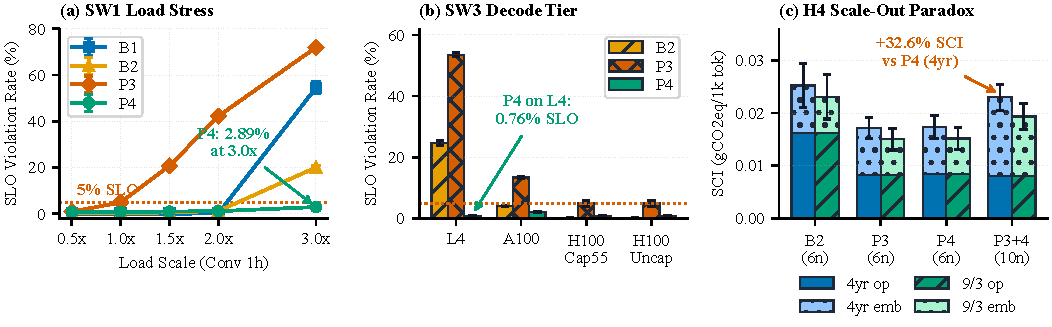
\includegraphics[width=\ifdefined\BUILDELSEVIER 0.94\textwidth\else 0.57\textwidth\fi]{figures/fig7_sw_sensitivity_embodied.pdf}
    \caption{Robustness and lifecycle evaluations ($N=10$ seeds, 95\% CIs): (a) \texttt{SW1} load scaling (\texttt{P4} holds 2.89\% at 3.0x); (b) \texttt{SW3} decode GPU tiers (\texttt{P4} holds 0.76\% on \texttt{L4}); (c) \texttt{H4} clean over-provisioning (+4 nodes) raising net $\text{SCI}_{\text{tot}}$ by +27.71\% to +32.61\%.}
    \label{fig:sw_paradox}
\end{figure*}

\subsection{Summary Answers to Research Questions (\texorpdfstring{\texttt{RQ1--RQ4}}{RQ1-RQ4})}\label{subsec:rq_answers}
\begin{itemize}
    \item \textbf{RQ1:} While GreenLLM~\cite{shi2024greenllm} handles single-cluster P/D carbon and multi-DC routers~\cite{topcu2026tension,moore2025slit,zhang2026context,bernhard2026cleanest} schedule colocated LLMs, 75.4\% of 61 works omit embodied carbon, 0/8 geo-routers use P/D or WAN KV gating, and 0 implemented systems unify all four axes with keep-alive.
    \item \textbf{RQ2:} Hybrid routing (\texttt{P4}) cuts \texttt{conv} $\text{SCI}_{\text{op}}$ by 60.70\%--60.77\% ($\text{SCI}_{\text{tot}}$ 54.64\%--54.92\%, $|r_{\text{rb}}|=1.000$) at $<1\%$ SLO violation and trims \texttt{P3} \texttt{code} SLO violations by 85.22\%--86.01\% by pruning Path C (0\%) to rely on Path D and local fallbacks.
    \item \textbf{RQ3:} GapHazard (\texttt{S3}) saves 7.03\%--11.02\% \texttt{TEPCO} $\text{SCI}_{\text{op}}$ (23.74\%--30.93\% for 48--84~s loaders) with 28.60\% SLO violations, yet flips to cut clean \texttt{South Scotland} SLO violations by 32.63\% vs.\ 30~s TTL.
    \item \textbf{RQ4:} Embodied carbon hits 93.0\%--97.6\% of clean-grid SCI, so four spare clean nodes raise net $\text{SCI}_{\text{tot}}$ by +32.61\% (4-yr) and +27.71\% (9~yr/3~yr).
\end{itemize}

\section{Open Challenges and Limitations}\label{sec:challenges}

\subsection{Synthesized Open Research Challenges (\texorpdfstring{\texttt{OC1--OC7}}{OC1-OC7})}\label{subsec:open_challenges}
Combining the literature gap matrix (Section~\ref{sec:taxonomy}) with the simulation trade-offs in Section~\ref{sec:results} identifies seven open research challenges:
\begin{itemize}
    \item \textbf{OC1 (Cross-Region KV-Cache Transport):} Even at 100~Gbps WAN, the carbon-and-latency gate prunes cross-region P/D transfers for over 99.9\% of arrivals. Closing that gap requires semantic token-level KV compression~\cite{jiang2026kvcache} integrated with live grid-carbon price gates.
    \item \textbf{OC2 (Live Marginal vs.\ Average Carbon Control):} Most cloud systems, including the baseline \texttt{E1} sweeps, optimize average regional grid intensity ($\text{gCO}_2\text{eq/kWh}$). Dispatching multi-megawatt LLM bursts requires marginal emission factors and grid-curtailment telemetry to reflect fossil peaker dispatch.
    \item \textbf{OC3 (Sub-Minute Embodied Cluster Sizing):} While per-request dispatch in \texttt{P4} minimizes operational carbon plus queue risk, \texttt{H4} shows that idle over-provisioning in clean zones reverses lifecycle gains (+32.6\% $\text{SCI}_{\text{tot}}$). Joint control planes must couple sub-second routing with hourly embodied scale-down and heterogeneous reuse (9~yr/3~yr lifetimes~\cite{li2025ecoserve,hewage2025aging}).
    \item \textbf{OC4 (Serverless Multi-Tenant Checkpoint Sharing):} On \texttt{TEPCO}, dynamic keep-alive still faces an 8.0\% vs.\ 28.60\% carbon-SLO squeeze. Page-shared GPU weight caching across concurrent LoRA adapters and MPS partitions~\cite{wang2026festina} can amortize 10.3~s NVMe cold starts across tenants.
    \item \textbf{OC5 (Water-Energy-Carbon Co-Optimization):} As CASA~\cite{qi2024casa} notes for serverless CPUs, shifting LLM inference purely toward dry wind/solar regions risks shifting cooling water stress unless water intensity enters Eq.~\eqref{eq:sci}.
    \item \textbf{OC6 (Bursty Code-Completion Admission Control):} Under $\text{CV} = 13.152$, no fixed 6-node strategy stayed below 5\% SLO violations without elastic spillover or prefill-priority admission pricing.
    \item \textbf{OC7 (Hardware Testbed Verification Across Continents):} Only 28.6\% of reviewed empirical systems pair testbeds with trace simulators, and none tests live WAN disaggregated LLM serving across continents (0/6); multi-continent hardware validation remains untested.
\end{itemize}

\subsection{Limitations and Threats to Validity}\label{subsec:limitations}
Several methodological constraints bound the interpretation of these results:
\begin{enumerate}
    \item \textbf{Simulation Abstraction vs.\ Physical Clusters:} Findings rely on analytical queueing and SimPy 4.1.2 discrete-event execution; no measurements come from instrumented multi-continent Kubernetes/vLLM deployments. Actual RDMA tail jitter, PCIe thermal throttling, and Linux memory fragmentation may shift absolute latency margins, although relative policy rankings (\texttt{P4} over \texttt{P3} and \texttt{B1}/\texttt{B2}) rest on structural bottlenecks observed in physical single-cluster studies~\cite{patel2024splitwise,zhong2024distserve,li2026revisiting}.
    \item \textbf{Calibrated Model Parameters:} Cross-region WAN RTT (20--200~ms), commodity WAN bandwidth (10--100~Gbps), sublinear MFU exponent ($\gamma=0.70$), and cold-start GPU power fraction ($f_{\text{cold}}=0.65$) are engineering assumptions bounded by published ranges (Table~\ref{tab:calibrations}) and not direct hardware measurements; \texttt{SW3} and \texttt{SW4} sweep these parameters across wide intervals.
    \item \textbf{24-Hour Trace Tiling:} Raw Azure LLM traces span 58.36 min (\texttt{conv}) and 57.27 min (\texttt{code})~\cite{azure2024trace}. Multi-day evaluations rely on block resampling across 24-hour UK/Japan grid curves while holding exact token distributions and arrival CVs constant.
    \item \textbf{Live Dispatch vs.\ Provisioning Scope:} Inside Eq.~\eqref{eq:dispatch}, per-request \texttt{P4} routing scores operational cost and queue pressure; hardware embodied amortization is evaluated across fixed versus over-provisioned cluster configurations (\texttt{H4\_elastic}) without dynamically powering servers on or off inside \texttt{E1}.
    \item \textbf{Corpus Access and Preprints:} Five works (10.6\%) could be verified only via abstracts~\cite{roy2026lowcarb,calavaro2026offloading,gupta2022act,sinha2025utilization,calheiros2011cloudsim}, and eight full-text works (17.0\%) are arXiv or accepted conference preprints (6 arXiv-only, 2 accepted preprints), which may undergo peer-reviewed revision prior to archival publication.
\end{enumerate}

\section{Conclusion}\label{sec:conclusion}

This work investigated the joint intersection of carbon-aware cloud/serverless scheduling and phase-disaggregated LLM serving through a PRISMA-2020-guided review of 61 studies (56 full-text, 5 abstract-only) and a hardware-validated SimPy 4.1.2 simulation driven by Azure, UK NESO, and Japan TSO traces. While recent systems tackle individual dimensions such as single-cluster P/D carbon/GPU reuse~\cite{shi2024greenllm} or colocated multi-region routing~\cite{topcu2026tension,moore2025slit,zhang2026context,bernhard2026cleanest}, 75.4\% of reviewed studies omit manufacturing carbon, 0/8 cross-region carbon schedulers model P/D disaggregation or WAN KV transport, and no implemented system jointly integrates all four control axes alongside serverless checkpoint keep-alive.

Trace-driven multi-seed simulations show that unconditional spatial disaggregation (\texttt{P3}) suffers tail collapse under bursty coding traffic (44.45\%--44.57\% SLO violations) and $3\times$ load spikes (71.94\%). Hybrid carbon-and-queue routing (\texttt{P4}) preserves 0.81\%--0.82\% SLO violations on conversational workloads while cutting operational SCI by 60.70\%--60.77\% and lifecycle SCI by 54.64\%--54.92\% relative to colocation ($|r_{\text{rb}}|=1.000$, $p=0.002$), and lowers \texttt{code} SLO violations by 85.22\%--86.01\% below \texttt{P3} by pruning cross-region Path C (0\%) in favor of Path D remote clean-grid execution and local Path A/B fallbacks. In serverless deployments, dynamic GapHazard keep-alive (\texttt{S3}) trims dirty-grid \texttt{TEPCO} operational SCI by 7.03\%--11.02\% (amplified to 23.74\%--30.93\% for slow 48--84~s loaders) while curbing clean-grid \texttt{South Scotland} SLO violations by 32.63\% below static 30~s timeouts. Finally, hardware amortization constitutes 93.0\%--97.6\% of clean-grid lifecycle emissions, causing four redundant clean nodes to raise net total SCI by +27.71\% to +32.61\%. Future physical testbeds should pair power-capped intra-region disaggregation with WAN KV compression, sub-minute clean-capacity sizing, and shared NVMe checkpoint pools.

\ifdefined\BUILDANON
\section*{Declaration of Generative AI Use}
Generative AI tools were used during manuscript preparation for literature search assistance, drafting, figure scripting, and language editing. Every reference, quantitative claim, simulator check, and figure was verified directly against primary sources and raw CSV outputs.

\section*{Data and Code Availability}
External datasets (Azure LLM Inference Traces and GreenSKU tables, UK NESO Carbon Intensity API, and Japan FY2024 TSO factors) are publicly available; simulator code, PRISMA records, and reproduction scripts are hosted in a repository omitted here (\repourl).
\else
\section*{Declaration of Generative AI Use}
Generative AI tools were used during the preparation of this manuscript for literature search assistance, drafting, figure generation, and language editing. I reviewed and verified all references, claims, simulation outputs, and figures directly against primary sources, and take full responsibility for the content of this paper.

\section*{Data and Code Availability}
All external workload and grid datasets are publicly available under CC-BY-4.0 licenses: Azure LLM Inference Traces and GreenSKU component tables via AzurePublicDataset (\url{https://github.com/Azure/AzurePublicDataset} and Zenodo \texttt{doi:10.5281/zenodo.10896254}), UK regional grid carbon intensity via the UK NESO Carbon Intensity API (\url{https://api.carbonintensity.org.uk}), and Japan FY2024 TSO emission factors via Zenodo (\texttt{doi:10.5281/zenodo.18396311}). The discrete-event simulator (SimPy 4.1.2), validation suite, PRISMA screening records, and figure-generation scripts are publicly available at \repourl.
\fi


\bibliographystyle{IEEEtran}
\bibliography{references}

\end{document}
